\subsection{UC5 - Modifica della riduzione dimensionale tramite calcolo delle distanze}
\begin{figure}[h]
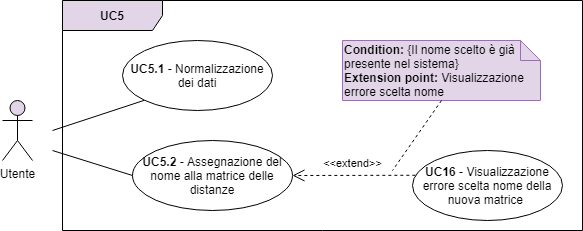
\includegraphics[width=17cm]{Section/Images/UC5.png}
\centering
\caption{UC5 - Modifica della riduzione dimensionale tramite calcolo delle distanze}
\end{figure}
\begin{itemize}
	\item \textbf{Attore primario}: Utente;
	\item \textbf{Precondizioni}: L'utente ha scelto la funzione per il calcolo delle distanze [UC3.2];
	\item \textbf{Postcondizioni}: I parametri necessari per creare la matrice delle distanze sono stati impostati;
	\item \textbf{Scenario principale}: L'utente:
	
	\begin{enumerate}
		\item Decide se attuare una normalizzazione ai dati prima di calcolare la distanza [UC5.1];
		\item Assegna un nome per identificare la matrice che verrà creata [UC5.2].
	\end{enumerate}		
\end{itemize}

\subsubsection{UC5.1 - Normalizzazione dei dati}

\begin{itemize}
	\item \textbf{Attore primario}: Utente;
	
	\item \textbf{Precondizioni}: L'utente ha scelto la funzione per il calcolo delle distanze [UC3.2];
	
	\item \textbf{Postcondizioni}: L'utente ha applicato una normalizzazione alle dimensioni selezionate;
	
	\item \textbf{Scenario principale}: L'utente seleziona la funzionalità di normalizzazione dei dati che sta analizzando.
\end{itemize}		

\subsubsection{UC5.2 - Assegnazione del nome alle dimensioni create}

\begin{itemize}
	\item \textbf{Attore primario}: Utente;
	
	\item \textbf{Precondizioni}: L'utente ha scelto la funzione per il calcolo delle distanze [UC3.2];
	
	\item \textbf{Postcondizioni}: L'utente ha assegnato il nome alla matrice delle distanze che andrà a creare;
	
	\item \textbf{Scenario principale}: L'utente assegna il nome alla matrice delle distanze che sta creando nell'apposito campo d'input. Se non modificato viene mantenuto il nome di default.
\item \textbf{Estensioni}:
	\begin{enumerate}[(a)]
		\item Nel caso in cui il nome scelto sia già stato utilizzato in precedenza:
		\begin{enumerate}[1.]
			\item La matrice delle distanze non viene creata;
			\item Viene visualizzato un errore esplicativo [UC16].
		\end{enumerate}
	\end{enumerate}
\end{itemize}	


\subsection{UC6 - Visualizzazione del dataset}
\begin{figure}[!htb]
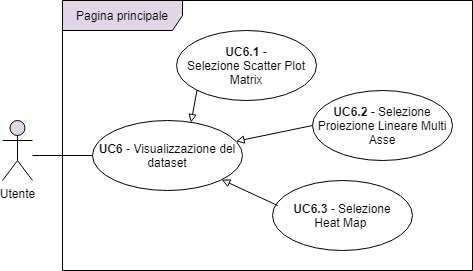
\includegraphics[width=14cm]{Section/Images/UC6.png}
\centering
\caption{Diagramma sul tipo di visualizzazione del dataset}
\end{figure}

\begin{itemize}
	\item \textbf{Attore primario}: Utente;
	\item \textbf{Precondizioni}: L'utente ha caricato dei dati nel sistema ed eventualmente effettuato una riduzione dimensionale tramite algoritmo [UC3.1];
	\item \textbf{Postcondizioni}: Viene mostrata la visualizzazione scelta, con possibilità di personalizzazione [UC8]. La scelta viene salvata nel sistema.
	\item \textbf{Scenario principale}: L'utente seleziona la visualizzazione che vuole utilizzare tra quelle disponibili.
	\item \textbf{Generalizzazioni}: L'utente seleziona una delle seguenti opzioni:
		\begin{enumerate}[(a)]
			\item \glo{\textit{Scatter Plot Matrix}} [UC6.1];
			\item \glo{\textit{Proiezione Lineare Multi Asse}} [UC6.2];
			\item \glo{\textit{Heat Map}} [UC6.3].
		\end{enumerate}

\end{itemize}

\subsubsection{UC6.1 - Selezione Scatter Plot Matrix}
\begin{itemize}
	\item \textbf{Attore primario}: Utente;
	\item \textbf{Precondizioni}: L'utente ha caricato dei dati nel sistema ed eventualmente effettuato una riduzione dimensionale tramite algoritmo [UC3.1];
	\item \textbf{Postcondizioni}: Viene mostrata la visualizzazione \glo{\textit{Scatter Plot Matrix}} scelta dall'utente, con possibilità di personalizzazione [UC8.1];
	\item \textbf{Scenario principale}: L'utente seleziona la visualizzazione \glo{\textit{Scatter Plot Matrix}} e il sistema ritorna un grafico con cui si può interagire.
\end{itemize}

\subsubsection{UC6.2 - Selezione Proiezione Lineare Multi Asse}

\begin{itemize}
	\item \textbf{Attore primario}: Utente;
	\item \textbf{Precondizioni}: L'utente ha caricato dei dati nel sistema ed eventualmente effettuato una riduzione dimensionale tramite algoritmo [UC3.1];
	\item \textbf{Postcondizioni}: Viene mostrata la visualizzazione \glo{\textit{Proiezione Lineare Multi Asse}} scelta dall'utente, con possibilità di personalizzazione [UC8.2];
	\item \textbf{Scenario principale}: L'utente seleziona la visualizzazione \glo{\textit{Proiezione Lineare Multi Asse}} e il sistema ritorna un grafico con cui si può interagire.
\end{itemize}

\subsubsection{UC6.3 - Selezione Heat Map}
\begin{itemize}
	\item \textbf{Attore primario}: Utente;
	\item \textbf{Precondizioni}: L'utente ha caricato dei dati nel sistema ed eventualmente effettuato una riduzione dimensionale tramite algoritmo [UC3.1];
	\item \textbf{Postcondizioni}: Viene mostrata la visualizzazione \glo{\textit{Heat Map}} scelta dall'utente, con possibilità di personalizzazione [UC8.3];
	\item \textbf{Scenario principale}: L'utente seleziona la visualizzazione \glo{\textit{Heat Map}} e il sistema ritorna un grafico con cui si può interagire.

\end{itemize}

\newpage

\subsection{UC7 - Visualizzazione basata sul concetto di distanza}
\begin{figure}[!htb]
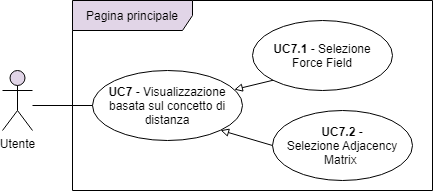
\includegraphics[width=13cm]{Section/Images/UC7.png}
\centering
\caption{Diagramma sul tipo di visualizzazione distance-based}
\end{figure}

\begin{itemize}
	\item \textbf{Attore primario}: Utente;
	\item \textbf{Precondizioni}: L'utente ha caricato dei dati nel sistema e ha generato una matrice delle distanze [UC3.2];
	\item \textbf{Postcondizioni}: Viene mostrata la visualizzazione scelta, con possibilità di personalizzazione [UC8]. La scelta viene salvata nel sistema;
	\item \textbf{Scenario principale}: L'utente seleziona la visualizzazione che vuole utilizzare tra quelle disponibili;
	\item \textbf{Generalizzazioni}: L'utente seleziona una delle seguenti opzioni:
		\begin{enumerate}[(a)]
			\item \glo{\textit{Adjacency Matrix}} [UC7.1];
			\item \glo{\textit{Force Field}} [UC7.2].
		\end{enumerate}

\end{itemize}

\subsubsection{UC7.1 - Selezione Adjacency Matrix}
\begin{itemize}
	\item \textbf{Attore primario}: Utente;
	\item \textbf{Precondizioni}: L'utente ha caricato dei dati nel sistema ed ha generato una matrice delle distanze [UC3.2];
	\item \textbf{Postcondizioni}: Viene mostrata la visualizzazione \glo{\textit{Adjacency Matrix}} scelta dall'utente, con possibilità di personalizzazione [UC8.2];
	\item \textbf{Scenario principale}: L'utente seleziona la visualizzazione \glo{\textit{Adjacency Matrix}} e il sistema ritorna un grafico con cui si può interagire.

\end{itemize}

\subsubsection{UC7.2 - Selezione Force Field}
\begin{itemize}
	\item \textbf{Attore primario}: Utente;
	\item \textbf{Precondizioni}: L'utente ha caricato dei dati nel sistema ed ha generato una matrice delle distanze [UC3.2];
	\item \textbf{Postcondizioni}: Viene mostrata la visualizzazione \glo{\textit{Force Field}} scelta dall'utente, con possibilità di personalizzazione [UC8.3];
	\item \textbf{Scenario principale}: L'utente seleziona la visualizzazione \glo{\textit{Force Field}} e il sistema ritorna un grafico con cui si può interagire.
\end{itemize}